\documentclass[11pt,border=5pt]{standalone}
\usepackage{fontspec}
\setmainfont{cmunrm.otf}[BoldFont=cmunbx.otf,ItalicFont=cmunti.otf,BoldItalicFont=cmunbi.otf]
\usepackage{amsmath}
\usepackage{unicode-math}
\setmathfont{NewCMMath-Regular.otf}
\usepackage{tikz}
\usetikzlibrary{arrows.meta,patterns,angles,quotes}
\begin{document}
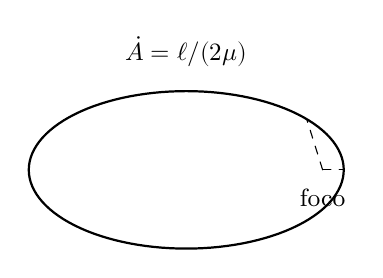
\begin{tikzpicture}[>=Stealth,font=\small,line cap=round,line join=round]
\draw[thick] plot coordinates {(2.00000,0.00000) (1.99726,0.05234) (1.98904,0.10453) (1.97538,0.15643) (1.95630,0.20791) (1.93185,0.25882) (1.90211,0.30902) (1.86716,0.35837) (1.82709,0.40674) (1.78201,0.45399) (1.73205,0.50000) (1.67734,0.54464) (1.61803,0.58779) (1.55429,0.62932) (1.48629,0.66913) (1.41421,0.70711) (1.33826,0.74314) (1.25864,0.77715) (1.17557,0.80902) (1.08928,0.83867) (1.00000,0.86603) (0.90798,0.89101) (0.81347,0.91355) (0.71674,0.93358) (0.61803,0.95106) (0.51764,0.96593) (0.41582,0.97815) (0.31287,0.98769) (0.20906,0.99452) (0.10467,0.99863) (0.00000,1.00000) (-0.10467,0.99863) (-0.20906,0.99452) (-0.31287,0.98769) (-0.41582,0.97815) (-0.51764,0.96593) (-0.61803,0.95106) (-0.71674,0.93358) (-0.81347,0.91355) (-0.90798,0.89101) (-1.00000,0.86603) (-1.08928,0.83867) (-1.17557,0.80902) (-1.25864,0.77715) (-1.33826,0.74314) (-1.41421,0.70711) (-1.48629,0.66913) (-1.55429,0.62932) (-1.61803,0.58779) (-1.67734,0.54464) (-1.73205,0.50000) (-1.78201,0.45399) (-1.82709,0.40674) (-1.86716,0.35837) (-1.90211,0.30902) (-1.93185,0.25882) (-1.95630,0.20791) (-1.97538,0.15643) (-1.98904,0.10453) (-1.99726,0.05234) (-2.00000,0.00000) (-1.99726,-0.05234) (-1.98904,-0.10453) (-1.97538,-0.15643) (-1.95630,-0.20791) (-1.93185,-0.25882) (-1.90211,-0.30902) (-1.86716,-0.35837) (-1.82709,-0.40674) (-1.78201,-0.45399) (-1.73205,-0.50000) (-1.67734,-0.54464) (-1.61803,-0.58779) (-1.55429,-0.62932) (-1.48629,-0.66913) (-1.41421,-0.70711) (-1.33826,-0.74314) (-1.25864,-0.77715) (-1.17557,-0.80902) (-1.08928,-0.83867) (-1.00000,-0.86603) (-0.90798,-0.89101) (-0.81347,-0.91355) (-0.71674,-0.93358) (-0.61803,-0.95106) (-0.51764,-0.96593) (-0.41582,-0.97815) (-0.31287,-0.98769) (-0.20906,-0.99452) (-0.10467,-0.99863) (-0.00000,-1.00000) (0.10467,-0.99863) (0.20906,-0.99452) (0.31287,-0.98769) (0.41582,-0.97815) (0.51764,-0.96593) (0.61803,-0.95106) (0.71674,-0.93358) (0.81347,-0.91355) (0.90798,-0.89101) (1.00000,-0.86603) (1.08928,-0.83867) (1.17557,-0.80902) (1.25864,-0.77715) (1.33826,-0.74314) (1.41421,-0.70711) (1.48629,-0.66913) (1.55429,-0.62932) (1.61803,-0.58779) (1.67734,-0.54464) (1.73205,-0.50000) (1.78201,-0.45399) (1.82709,-0.40674) (1.86716,-0.35837) (1.90211,-0.30902) (1.93185,-0.25882) (1.95630,-0.20791) (1.97538,-0.15643) (1.98904,-0.10453) (1.99726,-0.05234) (2.00000,-0.00000)};
\draw[dashed] (1.7320508075688772,0) -- (2,0);
\draw[dashed] (1.7320508075688772,0) -- (1.529684374568977,0.644217687237691);
\node at (1.7320508075688772,-0.35) {foco};
\node at (0,1.5) {$\dot A=\ell/(2\mu)$};

\end{tikzpicture}
\end{document}
